\section[Requisitos e Rastreabilidade]{Requisitos e Rastreabilidade}
A rastreabilidade pode ser definida como a habilidade de se acompanhar a vida
de um requisito em ambas as direções do processo de software e durante todo o ciclo de
vida. Ela fornece uma base para o desenvolvimento de uma trilha de auditoria para todo
o projeto, possibilitando encontrar outros requisitos e artefatos que podem ser afetados
pelas mudanças solicitadas (PALMER, 1997). 

Para tal, é necessário haver ligações entre requisitos e entre requisitos e outros elementos do processo de software. Assim, a identificação da composição de requisitos, das dependências entre requisitos, de
requisitos conflitantes, da origem dos requisitos e de seus interessados, além da
identificação de em quais artefatos produzidos durante o desenvolvimento de software
um requisito é tratado, é de fundamental importância para que a rastreabilidade possa
ser implementada (WIEGERS, 2003; ROBERTSON; ROBERTSON, 2006;
KOTONYA; SOMMERVILLE, 1998). 

A rastreabilidade se encaixa em nosso projeto de maneira bidirecional, onde é
possível rastrear a dependência entre os todos os níveis de abstração do projeto,
épicos, features e histórias de usuário.

Esse tipo de rastreabilidade deve tanto acontecer na forma horizontal quanto
na vertical. A rastreabilidade bidirecional é importante para analisar o impacto
de mudanças (em direção à implementação) e verificar a satisfação dos
requisitos (em direção à origem).

Embora a rastreabilidade de requisitos não possa ser completamente
automatizada, porque o conhecimento das ligações se origina na mente dos membros da
equipe de desenvolvimento, uma vez identificadas essas ligações, ferramentas de apoio
são importantíssimas para ajudar a gerenciar a grande quantidade de informações de
rastreabilidade (WIEGERS, 2003). 

Nas imagens que seguem logo abaixo, é possível visualizar tanto a rastreabilidade horizontal quanto a vertical. A primeira é a matriz de rastreabilidade do nosso projeto de forma macro, com todos os épicos, features e histórias de usuário. Portanto, representa a rastreabilidade horizontal do projeto.

Já a segunda imagem é um pouco mais restrita em informações: foi usado um filtro em features específicas. Na imagem em questão, destacam-se as features "Atribuir Aluno ao Contrato" e "Atribuir Aluno à Aulas". Nela é possível identificar as dependências entre as histórias de usuário, ou seja, representa a rastreabilidade vertical do projeto.

\begin{figure}[!htb]
    \centering
    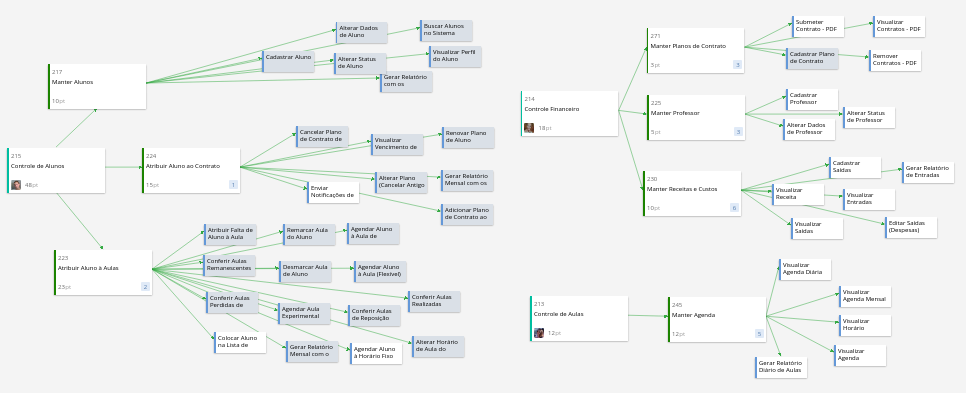
\includegraphics[width=1.4\textwidth, angle=-90]{figuras/matriz_rastreabilidade.png}
    \caption{Matriz de Rastreabilidade}
    \label{fig:matriz_rastreabilidade}
\end{figure}

\begin{figure}[!htb]
    \centering
    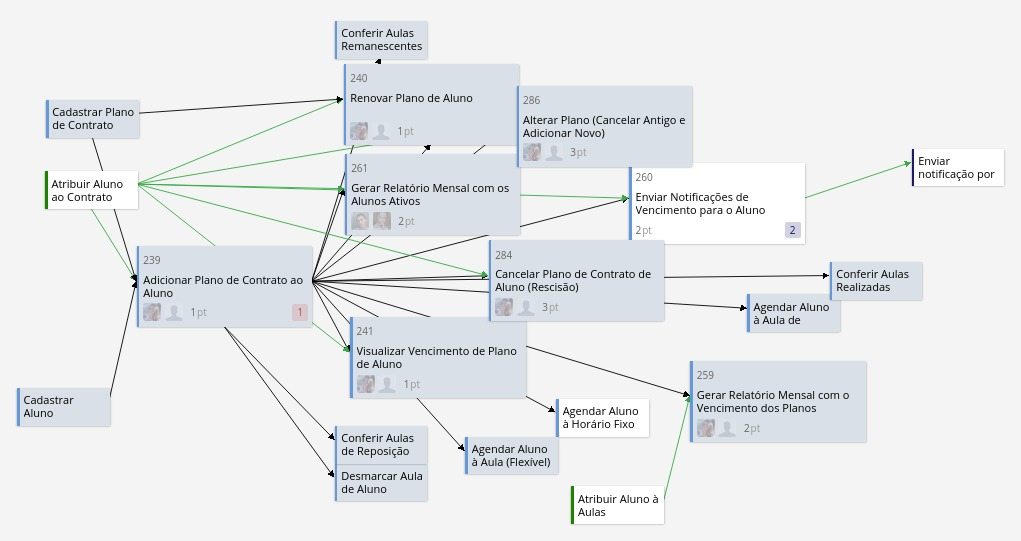
\includegraphics[width=\textwidth]{figuras/matriz_relacionamentos.jpeg}
    \caption{Matriz de Relacionamentos}
    \label{fig:matriz_relacionamentos}
\end{figure}
